\subsection{Resource Management and QoS}
\label{sec:qos}

Resource management and QoS have to be carefully coordinated. We use the term ``resource'' both for hardware, including computational, communication, and storage devices, and for data items such as data structures, blocks, objects, and files. To satisfy a request, the system has to locate resources that can satisfy the request: both devices and data items (or allocate the space for data items in case of writes).

\subsubsection{Resource Management}
Careful resource management strategies that can deal with placement and
retrieval of a large number of data items spread across the entire storage
hierarchy are key for predictable performance. 
%This connection is particularly important for data retrieval - in large scale
%storage systems, finding a resource to read can be a significant, if not
%dominant, component of overall read latency. 
Locating resources in a distributed system is a well-known problem: centralized
solutions suffer scalability challenges due to centralized, serialized system
updates. Many POSIX-compliant distributed file systems are good examples as updates to files require updates to their centrally maintained
metadata. %block allocation tables. 
% Carlos says: Parallel, POSIX-compliant file systems like Panasas,
% Lustre, and Ceph have never used central block allocation tables
% but only in local file systems they stripe over.
Distributed metadata management solutions on the other hand pose
challenges in keeping metadata management consistent and load-balanced
across different workloads~\cite{sevilla:sc15}. Methods to make
searches more efficient without reverting to centralized
bookkeeping usually involves search space partitioning and a method to limit
the search to a small number of partitions.  Frequently this involves a
hash function that is relatively stable against changes to its range, such as
failures or updates to the hardware of the system. Consistent
hashing~\cite{karger:stoc97} is scalable since it can be well-known throughout
a system of any size and only requires minimal movement of data in the presence
of failures or system changes. 
%Consistent hash functions can also have sets of ordered but infinite lists as
%their range (which works well with primary replication)
%~\cite{honicky:ipdps04}, implement declustering (limiting overlap between
%partitions), and support placement policy rules~\cite{weil:sc06}.

\paragraph{Approach:} In this proposal we introduce the concept of ``pile systems'' as a contrast to file systems. The name
is derived from personal information management user studies that divide users into ``pilers'' and ``filers''~\cite{malone:tois83}. More recent user studies showed that users generally use both piling and filing strategies, but to different degrees~\cite{whittaker:tochi01} (the lead author of this paper is now at UC Santa Cruz). Pile systems are systems that are capable of adding data with little ingest or metadata overhead or any placement restrictions and instead pay the cost of finding data at the time at which the data is retrieved. Pile systems are in contrast to file systems which maintain metadata and coordinate placement to minimize the cost of finding data. Pile systems enable efficient writes and flexible placement because clients can write wherever there
is free space with little bookkeeping overhead. However, pile systems can have unbounded search times, especially when it is unclear whether the resource actually exists. A good example of a pile system design is Sirocco which offers exceptionally flexible storage management.

% Sirocco offers more of a pile struture rather than a file structure. One of the
% challenges we face is offering performance predictability more similar to
% POSIX-compliant file systems while we take advantage of the distributed,
% flexible storage management offered by Sirocco.

In the proposed project, we will investigate the trade-off in terms of predictable
performance between ``filing'' and ``piling'' data, and we will
prototype combinations of filing and piling strategies in Sirocco.
The performance trade-off has a
parallel in data management where there are two alternative paths to achieve
knowledge. The analogue to filing is  to ``extract, transform, and load'' (ETL)
data into a warehouse paying an upfront ingest cost to achieve fast 
querying~\cite{vassiliadis:ijdwm09}.
The analogue to piling is to not pay any upfront cost and instead query the
raw data directly by using a data processing platform such as Hadoop.  Recent
work has found that the combination of these two techniques can be optimized to
perform better than any one technique alone~\cite{lefevre:sigmod14a} (this is work supported in part by the DOE DAMASC project). We
believe that a similar opportunity exists for combining filing and piling
approaches to achieve performance predictability without sacrificing too much
flexibility. Our additional challenge is incorporating both the storage tiers
and data utility.

More specifically, the coarseness of a search space partitioning limits the
search time within a partition, i.e., finely partitioned search spaces require
little or no search within a partition but offer little placement flexibility.
Partitioning can also be fine in one dimension and coarse in another to allow
flexibility where it is most needed while still ensuring fast finding. For
example, a hash function can finely partition a low storage tier but each
partition can extend across multiple tiers so that a search must occur in order
to find a resource on a particular tier. 

%Specifically, we will address the following research questions:
%\begin{tightItemize}
%  \item Can we make any guarantees in a scalable decentralized system?; 
% \item  What quality of service metrics can be make guarantees on in a scalable
%    way?;
%  \item What kind of error rates will we have in our estimation and what error
%    rates are acceptable?;
%  \item How much will the qos scheduler, admission control, manager cost in
%    terms of resources and time?;
%  \item  How do we make the scheduler scalable with the size of the system?
%\end{tightItemize}

\subsubsection{Quality of Service (QoS)}
Our ultimate goal, rather than just performance predictability, is to offer
predictable QoS for the storage system.
%Performance quality can be expressed in either relative or absolute
%terms. Examples of relative performance terms are ``fair'',
%``proportional'', or ``priority/class-based'' (``the higher the
%priority the better the service'' or ``1st class is better than
%2nd''). The key advantage of relative performance terms is that
%they are easy to implement. The key disadvantage is the difficulty
%of making any guarantees based on those implementations --
%even relative guarantees are mired by the well-known effect of
%priority inversion~\cite{lampson:cacm80}. Examples of absolute
%performance terms are ``rate-based'', ``soft real-time'', and
%``hard real-time''. The key advantage of absolute performance
%terms are that they enable the implementation of strong
%guarantees: absolute terms enable agreements between application
%tasks and storage that we call \emph{reservations} and that do not
%change meaning depending
%on the storage system's workload. The key challenge of absolute
%performance terms is that their implementation is non-trivial,
%especially in large-scale systems.
One of the key differentiating features this project offers is driving storage
decisions through QoS~\emph{reservations} rather than continuing the current
model of allowing applications to compete freely without restriction for part
or all of the storage resources. The current approach leads to interference
effects~\cite{lofstead:2010:io-variability,liu_hotstorage} that can greatly
impact I/O performance predictability. 
%Further, with the introduction of additional tiers in the
%storage stack, the performance variability will increase with greater
%competiion for limited high performance resources. 
%% Temporaily commented out the above sentence, because it may not be true for
%the next DOE systems. 
Unfettered, this competition can yield lower system and application performance
than if applications attempt to reserve storage resources thereby enabling the
storage system to reason over its performance in terms of reservations and
actual performance.  In the cases where an application arrives that needs to
run more urgently than any of the other already running applications, the
system can rapidly respond to it by reducing the amount of resources taken by
less urgent applications, allowing the urgent application to finish, and later
reverting back to the previous committed resource level for the rest.  This can
be automatically enforced via user- or administrator- specified
policies.

There are two fundamental causes that can impede the I/O performance in an
extreme-scale SSIO system. One is indirection, where layers of storage tiers
are employed either for performance and/or for scalability reasons.  The direct
consequence is that there could be multiple traversing paths from application
end to the data resting place, and more often than not, the I/O paths are not
under control under of any single authority. The other cause is shared
resources use. The best effort I/O request/response nature and lack of QoS
mechanisms imply that there is little expected performance guarantee.  Both
indirection and shared resources use contribute to a high probability of
imbalanced resources use and thus the occurrence of congestion and degraded
performance.

Consider this example demonstrating this disconnection will hurt system
performance. We launch 4096 processes with each process doing a single file I/O
operation against half of the Spider II file system at ORNL. The file traces
are analyzed to examine the utilization distribution of different components.
Figures (a), (b) and (c) show the resource usage distribution for OSTs (object storage
target), OSSes (object storage server),
and LNETs (Lustre Networking), respectively. We observe a significant usage variation
across components of any given type (e.g., OST, OSS or LNET). For example, some
OSTs are used more than 10 times while some others are never used
(corresponding to zero frequency count). Similarly, OSSes and LNETs show
significant usage imbalance under the default placement strategy.
Consequently, imbalanced resource utilization increases the contention at
certain components more than others.

% Don't know how to integrate this. Gary
%Given these insights, we advocate the idea that the infrastructure
%knowledge should find a way to relay to the upper layer for better
%and more effective use of resources. We think this is more pertinent
%and critical given the recent development of multi-tier storage and
%storage component heterogeneity.  There needs to be a way for
%application/middleware layer to gain more exposure of storage system
%for more intelligent processing logic.  One prime example of such
%exposed knowledge can be request/response time. To most applications,
%this is a black box. Profiling it at the upper layer is neither
%efficient nor effective, as it doesn't reflect cross-layer
%characteristics. However, Most of storage layer does keep a detailed
%profiling of such information. We therefore envision and propose a
%histogram-based request/response profiling API that application and
%middleware layer can leverage and make more informative decisions.


\begin{figure}[tbh]
  \centering
  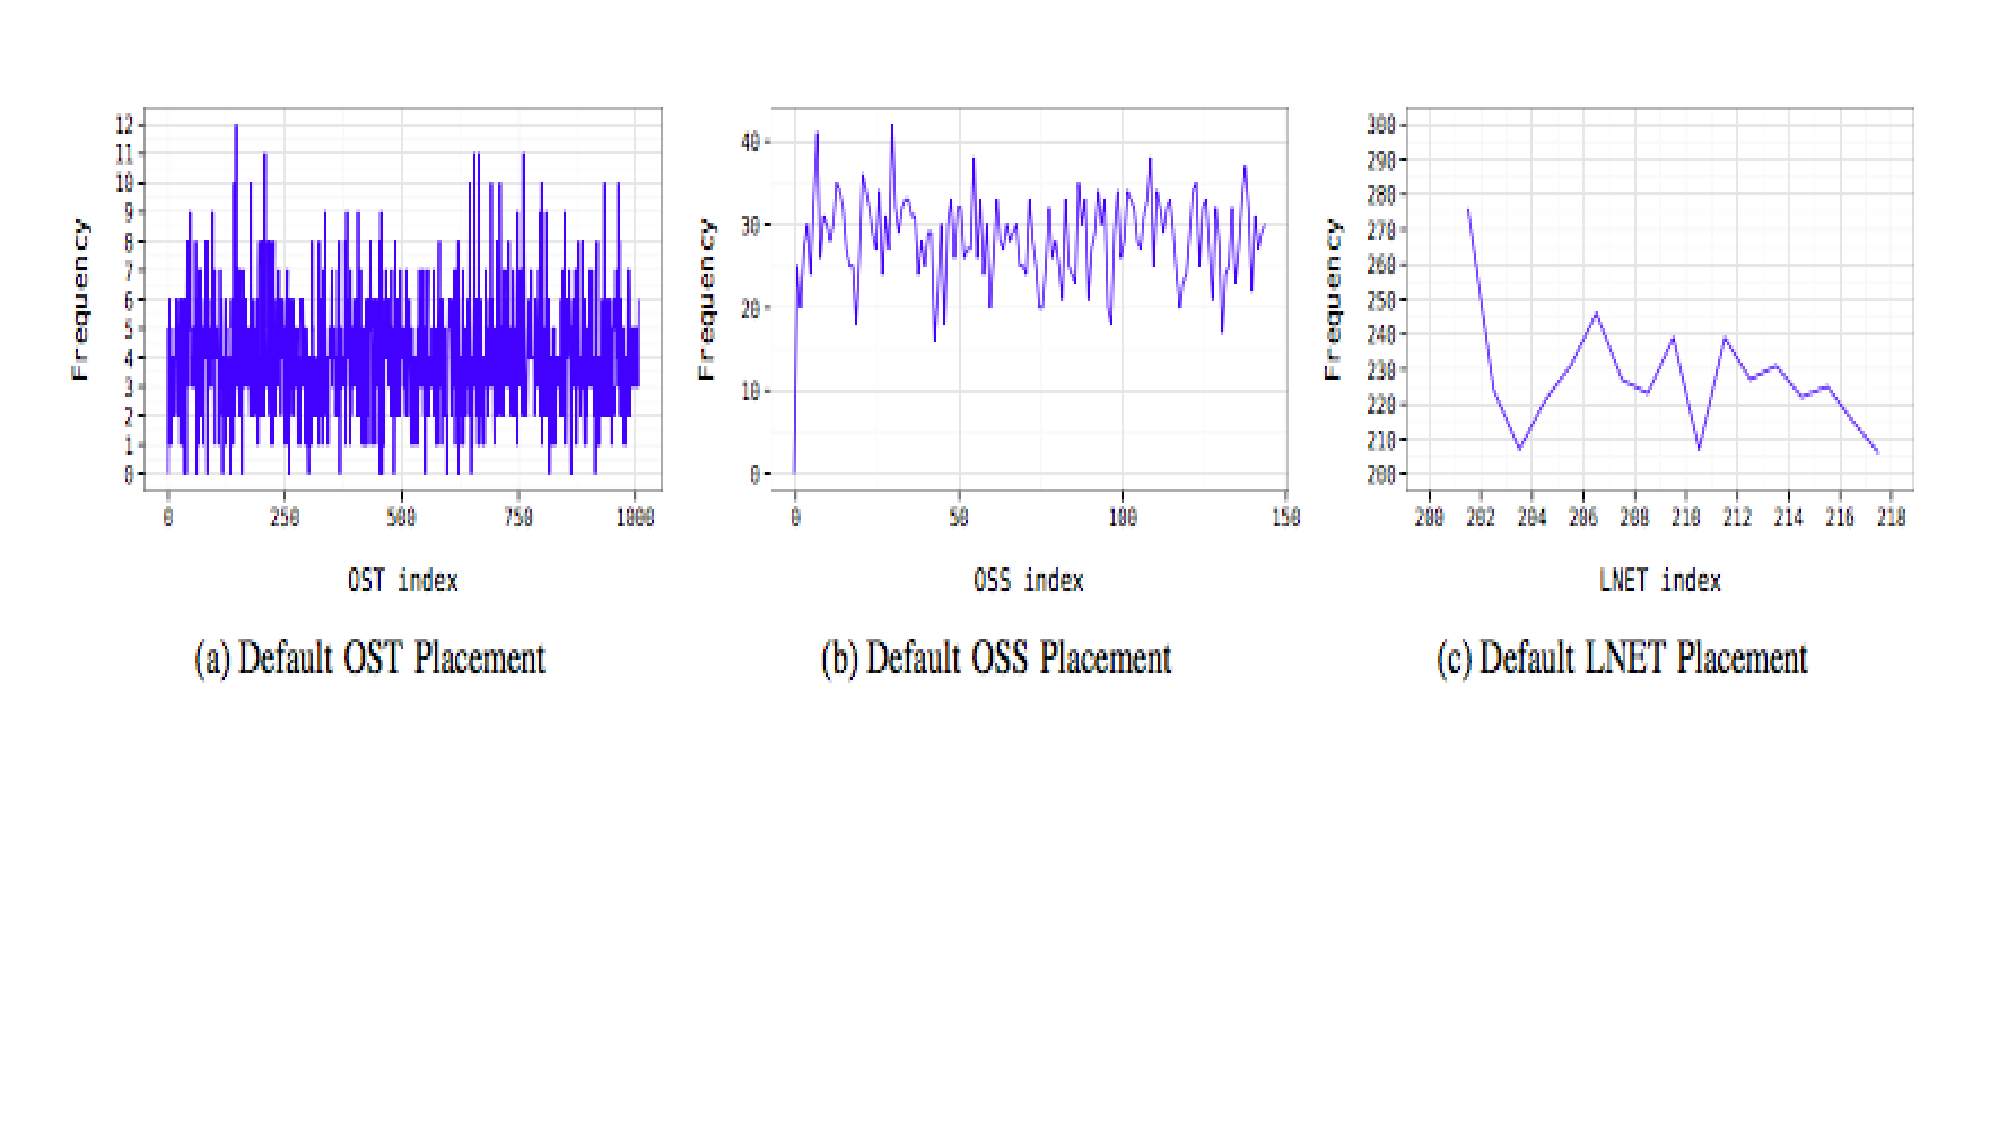
\includegraphics[width=\columnwidth]{graphics/infrastructure.pdf}
  \caption{Resource usage distribution for OST(a), OSS(b) and LNETs(c) }
\end{figure}
 \vspace{-2ex}


% This is about finding the relationshiop of workload-dependent to
% workload-independent metrics. -- Carlos
%are driven from multiple different approaches. First, supporting
%capability runs is a priority for capability machines. We propose to address
%capability run performance by incorporating monitoring for prepartory runs at
%smaller scale to profile the application output characteristics both from a
%writing velocity and volume, but also for example read patterns for the data
%analytics required to generate scientific insights from the raw data. 

% Not sure how to reuse this ... -- Carlos
%By
%discovering approximate data proportions that will likely be the key subsets
%targeted by the simulation run, we can generate a policy to preserve a certain
%storage portion for high fidelity data storagae and use slower or perhaps lower
%fidelity or compressed data storage for less interesting data portions. We will
%support spreading data appropriately across the storage hierarchy. In
%particular, we will investigate how to place data across different layers to
%meet the performance requirements for output while maintaining system
%availability for other applications and offering the best possible performance
%for the data analytics that will ultimately process this data.


% Not sure how to reuse this... -- Carlos
%Second, once data has been placed for future performance requirements, policies
%must be able to address maintaining data on a priority basis in that location
%to deliver on the placement optimization generated by the capability run
%profilier.

% This is a matter of metering, not performance reservations. -- Carlos
%Third, most future NVM devices have limited write endurance prompting
%management to ensure fair use by all machine users. Technologies like
%NAND-flash and Phase Change Memory have limited write endurance. By
%incorporating policies about the proportion of write endurance a compute
%allocation is entitled to, data placement decisions can be made to ensure fair
%resource usage. While the offending application will suffer worse IO
%performance, other applications that more carefully address their data
%intensity on these limited devices will achieve higher overall performnce. Only
%by instituting such policies can we encourage application users to adopt
%technology to manage the limited resources.


%We propose to investigate both offering a policy mechanism and how to implement
%these kinds of policies in a way that addresses offering the shortest
%end-to-end time for scientific insights.

% Lifted the following paragraph to the beginning. Gary
%``Quality of Service'' (QoS) refers to the
%properties of the performance qualtiy of a particular service, in
%this case the storage system.
%Performance quality can be expressed in either relative or absolute
%terms. Examples of relative performance terms are ``fair'',
%``proportional'', or ``priority/class-based'' (``the higher the
%priority the better the service'' or ``1st class is better than
%2nd''). The key advantage of relative performance terms is that
%they are easy to implement. The key disadvantage is the difficulty
%of making any guarantees based on those implementations --
%even relative guarantees are mired by the well-known effect of
%priority inversion~\cite{lampson:cacm80}. Examples of absolute
%performance terms are ``rate-based'', ``soft real-time'', and
%``hard real-time''. The key advantage of absolute performance
%terms are that they enable the implementation of strong
%guarantees: absolute terms enable agreements between application
%tasks and storage that we call \emph{reservations} and that do not
%change meaning depending
%on the storage system's workload. The key challenge of absolute
%performance terms is that their implementation is non-trivial,
%especially in large-scale systems.

\paragraph{Approach:}
The goals of this proposal require applications to demand guarantees in terms
of absolute performance qualities.  The first key enabler for any service to
make absolute guarantees is \emph{performance isolation}, i.e., the ability to
shield the performance impact of one task from another. The most
straight-forward but least flexible strategy is to simply cap the latency of
each task, regardless of its completeness (see for
example~\cite{decandia:sosp07}). This strategy is applicable when incomplete
tasks still have value and missing results are either not important or can be
easily retrieved in subsequent tasks. A more generally applicable strategy is
to control task admission to the system. \emph{Admission control} maintains a
\emph{utilization model} that can predict the utilization of system
resources given a new task, estimates the current utilization of the system,
and decides whether the task can be admitted without overloading the system.
Thus, admission control avoids system overload conditions that lead to
hard-to-model chaotic behaviors.  Consequently, utilization models can
frequently be approximated by automatically calibrated linear models (see for
example~\cite{skourtis:hpdc12}).

Another essential component of performance isolation is the \emph{charging
model} that determines which task(s) should be charged how much for a request.
Performance isolation is implemented by the charging model by ensuring that
task performance only depends on its reservation and its workload behavior (but
not on other workloads in the system). Each task has a budget based on its
reservation and spends it based on the cost of each request determined by the
charging model. A charging model determines the cost based on the utilization
model and the interactions a request can have with other requests (e.g. a
random request to spinning media interrupting a stream of sequential
requests). Thus users with a higher allocation can still meet their higher
requirements for I/O, without violating the gurantees given to other users. 

Performance isolation, including its utilization and charging models,
critically depends on \emph{workload-independent metrics}. Even though
throughput and latency are frequently the most meaningful metrics for an
application, they are not workload-independent and therefore are inadequate for
measuring device utilization across all workloads unless one accepts
worst-case estimates that can lead to gross resource underutilization. For
example, the throughput of random and sequential workloads in spinning media
differ by orders of magnitudes. A common workload-independent metric is
\emph{time utilization}, i.e., the amount of time a resource is utilized in a
given time interval. Time utilization has the advantage of having an always
defined maximum and therefore makes resources fully reservable. Even though a
workload-independent metric might at first not appear meaningful for an
application, given a particular workload an application can discover the
relationship between its workload-dependent metric and the workload-independent
metric.  Because of performance isolation, the application has to discover this
relationship only once.  To achieve effective performance isolation, we seek to
expand the resource management capabilities in Sirocco to support additional
utilization metrics to guide resource management decisions. Currently, Sirocco
offers automatic resource management capabilities, based on resource capacity
and data resilience requirements, and it needs to be extended to offer
data-centric metrics that help guide the forced QoS decisions.

% As stated in the introduction, we seek to make a storage stack that works with
% the user. Towards that end, we must incorporate data attributes into this
% process. For example, particularly for a capability run, the storage system
% should give (on a user by user basis), higher priority to data subset tagged with high importance to stay in fast
% storage tier
% administrators.
%  It should also store the highest value data possible given
% the performance requirement. Ideally, the storage system will store the raw
% data at full fidelity. 
% When this tier approaches capacity, data should migrate
% not just based on age, but also based on this value. One area of research will be in
% trying to see if we can retain some guarantees of QoS while providing
% policies that can govern admissio
% greater SSIO a higher {\bf priority} than other users on the system. 
% We realize that this makes
% it very difficult to main overall system QoS, but we will investigate techniques when one
% user is running on the majority of the exascale resource and we can allow them to lock out other SSIO
% request during small periods of time during the lifetime of their exascale simulation.


\paragraph{Related Work:}
On current production HPC systems, absolute I/O performance guarantees are not
possible. Previous work~\cite{lofstead:2010:io-variability,liu_hotstorage} from
this project team uses a client-assisted approach to mitigate I/O variablity at
scale (100,000-core).  Recently, server side QoS scheduling has also been
studied for HPC applications~\cite{Dai:2014,msst2012,vPFS-TOS}.  However, the key hurdle of
scalability has not been solved.  Existing efforts on scheduing
resources~\cite{thapaliya:2014:io-cop,dorier:2014:calciom} attempt to offer
admission control to maximize storage performance. Unfortunately, these efforts
are limited to participating applications and only applications from a single
platform. For this approach to be effective, the storage system must offer an
approach that handles clients from all connected platforms and does not require
modification to use new storage access APIs. By using a {\it value} tagging
system, we will offer defaults suitable for all applications that can be
informed by simple extensions to the job scheduler or more advanced management
through new APIs. On the other hand, storage QoS has been studied for
enterprise applications and systems~\cite{Gulati:2007,Gulati:2010,Gulati:2012}
in virtualized environments. It is not straightforward to adapt these solutions
to HPC storage systems because of the scalability and efficiency concerns,
despite they achieved very good performance isolations.

\paragraph{Challenges:}
The deep and heterogeneous memory and storage hierarchy we are assuming for
this proposal complicates the relationship between workload-dependent and
workload-independent metrics: the performance of a task can significantly
differ depending on what levels of the hierarchy are involved. Furthermore, an
important goal of the proposed project is to enable applications to reason
about the trade-off between accuracy and performance, adding yet another
dimension to how tasks are mapped to resources.

\begin{tightItemize}

\item A key challenge of admission control is scalability: the
decision of whether to admit a task could potentially depend on
global knowledge of the current utilization of every single resource
in the system. Scalability therefore depends on whether admission
control is able to accurately map a new task to a relatively small
set of resources which can quickly provide up-to-date utilization.
One approach might involve pseudo-random mapping that also load-balances
as a side-effect.

\item To offer performance and accuracy trade-offs, the system must be able
to quickly generate a number of data production plans, involving
different parts of the hierarchy and different data accuracy.
It will then use the utilization model to estimate the performance for
each production plan and the accuracy they can provide. Here
again, pseudo-random selection could reduce the number of resources
that would be involved, thereby increasing scalability.

\item The complexity of a utilization model involving the entire
storage hierarchy with 100,000s of devices is potentially daunting.
However, the utilization model can be simplified by modeling classes
of devices as well as classes of requests. In particular, each
device could restrict access to its content via a set of well-defined
methods with known, absolute performance properties.

\item Flash devices become inherently unpredictable when reads and
writes are mixed on the same device because of garbage collection.
While write latency can be easily hidden using asynchronous I/O,
hiding read latency is more difficult. By separating reads and
writes for each device, read latency becomes predictable. The
challenge is to minimize duplication of data, at least on fast
layers and leverage redundancy across layers.

\end{tightItemize}


%%% Local Variables:
%%% mode: latex
%%% TeX-master: "../proposal"
%%% End:

